\subsection{Hàm đa thức}

\ % Lùi đầu dòng

Một dạng hàm quen thuộc, được giới thiệu trong chương trình học trung học phổ thông, là đa thức, thông thường được biểu diễn dưới dạng $$f(x)=P_n(x)=\sum_{i = 0}^n a_i x^i = a_nx^n + a_{n-1}x^{n-1} + \cdots + a_1x + a_0$$ với $n$ là một số nguyên không âm, $a_i$ là các số thực, gọi là các \emph{hệ số}, với mọi $i$ nguyên nằm trong đoạn $[0, n]$ và $a_n \neq 0$. Khi này, $n$ được gọi là \emph{bậc} của đa thức\label{def:ham_so_mot_bien:da_thuc:da_thuc}. Mọi giá trị $x \in \mathbb{R}$ đều thuộc tập xác định của hàm đa thức $f(x)$. Ví dụ:
\begin{itemize}
   \item $f(x) = 2x^2 + 3x + 1$ là một đa thức bậc $2$ với các hệ số $a_2 = 2$, $a_1 = 3$, $a_0 = 1$;
   \item $g(y) = y^3 - 4y$ là một đa thức bậc $3$ với các hệ số $b_3 = 1$, $b_2 = 0$, $b_1 = -4$, $b_0 = 0$;
   \item $h(z) = 5$ là một đa thức bậc $0$ với hệ số $c_0 = 5$;
\end{itemize}
Tính toán một số giá trị mẫu:
\begin{itemize}
   \item $p(1) = 7 \cdot 1^4 - 2 \cdot 1^2 + 9 = 14$ với $q(t)= 7t^4 - 2t^2 + 9$ là một đa thức bậc $4$ với các hệ số $d_4 = 7$, $d_3 = 0$, $d_2 = -2$, $d_1 = 0$, $d_0 = 9$;
   \item $q(2) = -3 \cdot 2 + 8 = 2$ với $q(r) = -3r + 8$ là một đa thức bậc $1$ với các hệ số $e_1 = -3$, $e_0 = 8$.
\end{itemize}
Khi đa thức có bậc bằng $0$, hay $f = P_0 = a_0$, thì được gọi là \emph{đa thức hằng} hay \emph{hàm hằng}. Một trường hợp đặc biệt là khi $f = 0$ (hay $f(x) = 0$ với mọi $x$). Nếu hàm này là đa thức, theo định nghĩa, hàm này chỉ có duy nhất hệ số đầu $a_0 = 0$. Tuy nhiên, cũng theo định nghĩa thì hệ số đầu phải khác $0$. Vì vậy, hàm không có bậc và không được gọi là đa thức. Nhưng, do hàm nhận giá trị cố định với mọi $x$ nên vẫn được gọi là hàm hằng \footnote{Đa số những nhà toán học không coi $f = 0$ là đa thức bậc $0$ do nhiều tính chất của đa thức bị phá vỡ khi gặp trường hợp này. Tuy nhiên, nhiều người vẫn coi $f = 0$ là đa thức không có bậc. Trong tài liệu này, tác giả không coi $0$ là đa thức, nhưng vẫn coi là hàm hằng.}.

\exercise Phác thảo đồ thị của những hàm sau:
\begin{multicols}{2}
\begin{enumerate}
   \item $f(x) = x + 2$; 
   \item $f(x) = x^2 + 2x + 3$;
   \item $f(x) = x^3 - 9x^2 + 24x - 16$;
   \item $f(x) = 2$.
\end{enumerate}
\end{multicols}

\solution

Bạn đọc có thể dùng những phần mềm vẽ đồ thị để nhanh chóng có hình vẽ. Tuy nhiên, nếu không có thiết bị điện tử thì bạn đọc vẫn có thể vẽ đồ thị bằng giấy và bút bằng cách lấy nhiều điểm ví dụ cho $x$ và tính toán giá trị $f(x)$ và sau đó nối chúng lại với nhau.

Bạn đọc có thể để ý rằng là không phải lúc nào cũng đặt gốc tọa độ ở vị trí chính giữa. Trong nhiều trường hợp việc đặt chính giữa sẽ làm mất đi đồ thị và làm cho đồ thị lệch ra khỏi khu vực vẽ. Hơn nữa, hai trục sẽ có tỉ lệ khác nhau. Điều quan trọng nhất của những bài vẽ đồ thị trong vật lí không phải là căn ke chính xác vị trí từng điểm, mà là nhận ra được dáng điệu của đồ thị và vị trí tương đối giữa các điểm trên đồ thị đó. Qua đó, chúng ta rút ra được những tính chất toán học cần thiết để phục vụ những yêu cầu cụ thể trong bài tập ứng dụng.

Dưới đây là đồ thị của các hàm đa thức trong bài:

\begin{figure}[H]
   \centering
   \begin{minipage}[b]{0.48\textwidth}
      \centering
      \fbox{
         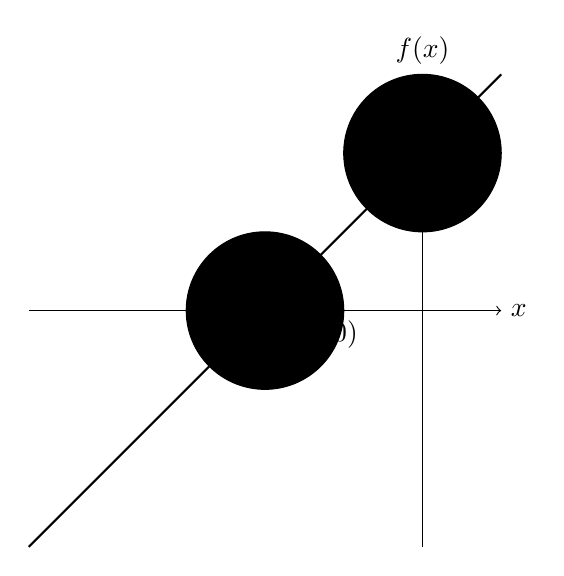
\begin{tikzpicture}
            \draw[->] (-5, 0) -- (1, 0) node[right] {$x$};
            \draw[->] (0, -3) -- (0, 3) node[above] {$f(x)$};
            \draw[thick] plot[domain=-5:1] (\x, {\x + 2});
            \filldraw (0, 2) circle (\pointSize) node[below right] {$\left(0; 2\right)$};
            \filldraw (-2, 0) circle (\pointSize) node[below right] {$\left(-2; 0\right)$};
         \end{tikzpicture}
      }
      \caption{Đồ thị của hàm $f(x) = x + 2$}
      \label{fig:ham_so:ham_da_thuc:x_2}
   \end{minipage}
   \hfill
   \begin{minipage}[b]{0.48\textwidth}
      \centering
      \fbox{
         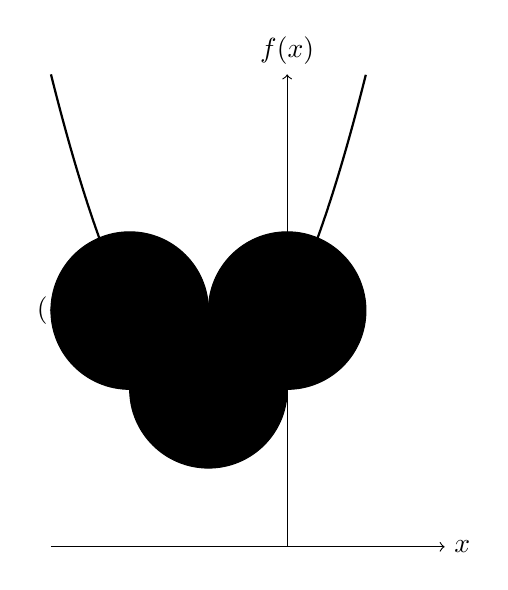
\begin{tikzpicture}
            \draw[->] (-3, 0) -- (2, 0) node[right] {$x$};
            \draw[->] (0, 0) -- (0, 6) node[above] {$f(x)$};
            \draw[thick, smooth, samples=100] plot[domain=-3:1] (\x, {(\x + 1)^2 + 2});
            \filldraw (-1, 2) circle (\pointSize) node[below] {$\left(-1; 2\right)$};
            \filldraw (0, 3) circle (\pointSize) node[below right] {$\left(0; 3\right)$};
            \filldraw (-2, 3) circle (\pointSize) node[left] {$\left(-2; 3\right)$};
         \end{tikzpicture}
      }
      \caption{Đồ thị của hàm $f(x) = x^2 + 2x + 3$}
      \label{fig:ham_so_mot_bien:da_thuc:x2_2x_3}
   \end{minipage}
\end{figure}
\begin{figure}[H]
   \centering
   \begin{minipage}[t]{0.48\textwidth}
      \centering
      \fbox{
         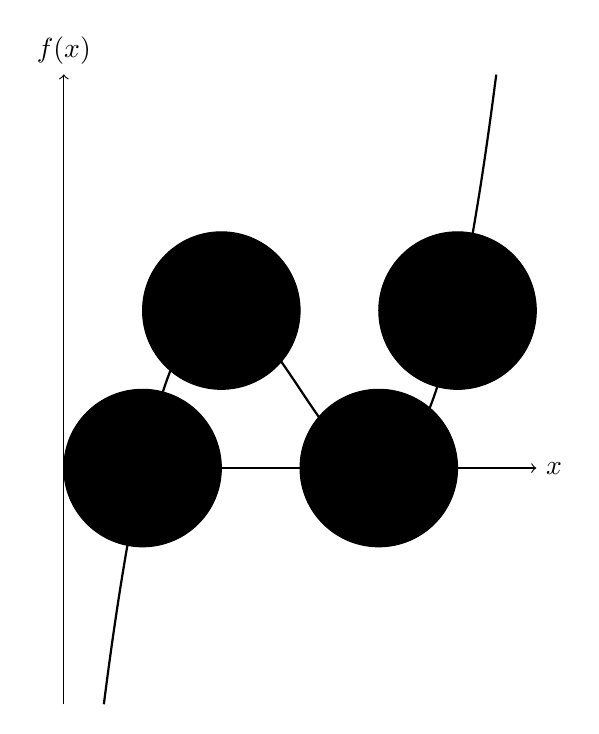
\begin{tikzpicture}
            \draw[->] (0, 0) -- (6, 0) node[right] {$x$};
            \draw[->] (0, -3) -- (0, 5) node[above] {$f(x)$};
            \draw[thick, smooth, samples=100] plot[domain=0.508:5.492] (\x, {((\x)^3 - 9*(\x)^2 + 24*(\x) - 16) / 2});
            \filldraw (2, 2) circle (\pointSize) node[above] {$\left(2; 4\right)$};
            \filldraw (4, 0) circle (\pointSize) node[below] {$\left(4; 0\right)$};
            \filldraw (1, 0) circle (\pointSize) node[below right] {$\left(1; 0\right)$};
            \filldraw (5, 2) circle (\pointSize) node[right] {$\left(5; 4\right)$};
         \end{tikzpicture}
      }
      \caption{Đồ thị của hàm $f(x) = x^3 - 9x^2 + 24x - 16$}
      \label{fig:ham_so_mot_bien:da_thuc:x3_t9x2_24x_t16}
   \end{minipage}
   \hfill
   \begin{minipage}[t]{0.48\textwidth}
      \centering
      \fbox{
         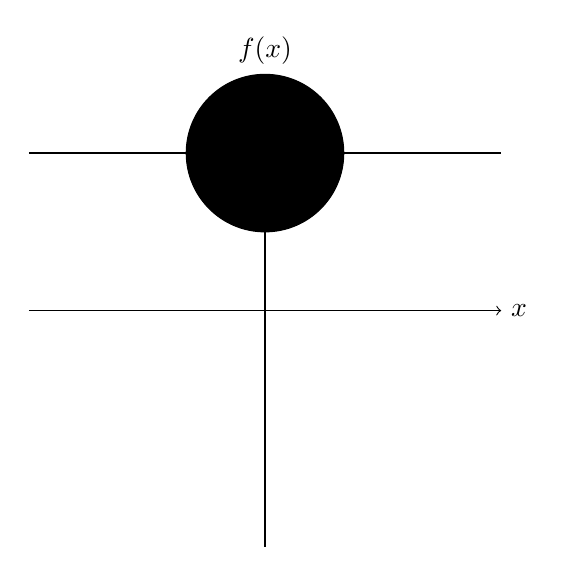
\begin{tikzpicture}
            \draw[->] (-3, 0) -- (3, 0) node[right] {$x$};
            \draw[->] (0, -3) -- (0, 3) node[above] {$f(x)$};
            \draw[thick] plot[domain=-3:3] (\x, {2});
            \filldraw (0, 2) circle (\pointSize) node[above left] {$\left(0; 2\right)$};
         \end{tikzpicture}
      }
      \caption{Đồ thị của hàm $f(x) = 2$}
      \label{fig:ham_so:ham_da_thuc:2}
   \end{minipage}
\end{figure}

\exercise Giải những phương trình sau. Các phương trình đều có ẩn là $x \in \mathbb{R}$.
\begin{multicols}{2}
   \begin{enumerate}
      \item $3x - 7 = 0$;
      \item $x - 9 = 5x + 3$;
      \item $\frac{1}{v}\cdot x - \frac{1}{v} \cdot x_0 = t$, với $v$, $x_0$, $t$ là những tham số thực;
      \item $6x^2 - 5x - 21 = 0$;
      \item $5x^2 - 50x + 125 = 0$;
      \item $x^2 + 2x + 4 = 0$;
      \item $x^2 + 2x + 4 = 8$;
      \item $5x^2 - 20x + 20 = x^2 - 4$;
      \item $\frac{1}{2}kx^2 + \frac{1}{2}mv^2 = \frac{1}{2}kx_0^2$, với $k$, $m$, $v$, $x_0$ là những tham số thực;
      \item $x^3 - \frac{11}{6}\cdot x^2 + x - \frac{1}{6} = 0$;
      \item $2x^3 - 2x^2 + 2x - 2 = 6 + 6x^2$.
   \end{enumerate}
\end{multicols}

\solution

1. Biến đổi tương đương phương trình để có:
\begin{align*}
   3x - 7 &= 0 \\
   \iff 3x &= 7\\
   \iff x &= \frac{7}{3}.
\end{align*}
Vậy tập nghiệm của phương trình là $\boxed{\displaystyle\left\{\frac{7}{3}\right\}}$.

2. Chuyển số hạng có thừa số $x$ về một phía, và số hạng tự do về phía còn lại để được:
\begin{align*}
   x - 9 &= 5x + 3 \\
   \iff (x - 9) + (9 - 5x) &= (5x + 3) + (9 - 5x) \\ 
   \iff -4x &= 12 \\
   \iff x &= -3.
\end{align*}
Vậy tập nghiệm của phương trình là $\boxed{\displaystyle\left\{-3\right\}}$.

3. Để giải phương trình có chứa tham số, chúng ta cần viết lại ẩn $x$ dưới dạng một biểu thức chỉ chứa tham số và hằng số. Cụ thể,
\begin{align*}
   \frac{1}{v}\cdot x - \frac{1}{v} \cdot x_0 &= t \\
   \iff \frac{x}{v} &= t + \frac{x_0}{v} \\
   \iff x &= vt + x_0.
\end{align*}
Vậy nghiệm của phương trình là $\boxed{\displaystyle\left\{vt + x_0\right\}}$.

4. Nếu như bạn đọc chưa biết, nếu như một đa thức $f(x)$ nhận $x = a$ là nghiệm thì $f(x)$ có thể được viết thành tích của $(x - a)$ nhân một đa thức $g(x)$ với bậc nhỏ hơn $1$ so với $f(x)$. Và nếu $g(x)$ lại có nghiệm $x = b$ thì chúng ta có thể viết $g(x) = (x-b)h(x)$ và qua đó có thể viết lại $f(x) = (x-a)(x-b)h(x)$. Một cách tổng quát nhất, nếu như $f(x)$ là phương trình bậc $n$ có $n$ nghiệm $a_1, a_2, \cdots, a_n$ thì có thể viết lại $$f(x) = A \prod_{i=1}^{n} (x - a_i) = A(x - a_1)(x - a_2)\cdots (x - a_n)$$ với $A$ là hệ số của số hạng có bậc lớn nhất trong đa thức $f(x)$.

Nhẩm nghiệm (bằng cách bấm máy tính) phương trình thì có $x = -\frac{3}{2}$ và $x = \frac{7}{3}$. Chúng ta kì vọng có thể viết lại phương trình dưới dạng $6\left(x - \left(-\frac{3}{2}\right)\right)\left(x - \frac{7}{3}\right) = 0$. Thực vậy, thực hiện phân tích nhân tử để có:
\begin{align*}
   &6x^2 - 5x - 21 = 0 \\
   \iff &6x^2 - 14x + 9x - 21 = 0 \\
   \iff &2x(3x - 7) + 3(3x - 7) = 0 \\
   \iff &(2x + 3)(3x - 7) = 0 \\
   \iff &\left[
      \begin{aligned}
         2x + 3 &= 0 \\
         3x - 7 &= 0
      \end{aligned}
   \right.
   \iff \left[
      \begin{aligned}
         x &= -\frac{3}{2} \\
         x &= \frac{7}{3}
      \end{aligned}
   \right..
\end{align*}
Vậy phương trình có nghiệm là $\boxed{\displaystyle\left\{-\frac{3}{2}; \frac{7}{3}\right\}}$.

5.
\begin{align*}
   5x^2 - 50x + 125 &= 0 \\
   \iff 5\left(x^2 - 10x + 25\right) &= 0 \\
   \iff 5(x - 5)^2 &= 0 \\
   \iff x - 5 &= 0 \\
   \iff x &= 5.
\end{align*}

Vậy tập nghiệm của phương trình có một phần tử duy nhất $\boxed{\displaystyle\left\{5\right\}}$.

6. Với những phương trình liên quan tới đa thức bậc hai không thể nhẩm ngay được nghiệm, chúng ta sẽ sử dụng phương pháp tách bình phương. Với phương trình được cho:
\begin{align}
   x^2 + 2x + 4 &= 0 \nonumber\\ 
   \iff x^2 + 2x + 1 &= -3 \nonumber\\
   \iff (x + 1)^2 &= -3. \label{eq:ham_so_mot_bien:ham_da_thuc:gptdt6}
\end{align}
Một số thực nhân với chính nó sẽ ra một số không âm. Cho nên phương trình \ref{eq:ham_so_mot_bien:ham_da_thuc:gptdt6} không thể đúng. Vậy phương trình \fbox{vô nghiệm} trên tập số thực.

7. 
\begin{align*}
   &x^2 + 2x + 4 = 8 \\ 
   \iff &x^2 + 2x + 1 = 5 \\
   \iff &(x + 1)^2 = 5 \\
   \iff &\left[
      \begin{aligned}
         x + 1 &= \sqrt{5} \\
         x + 1 &= -\sqrt{5}
      \end{aligned}
   \right. \\
   \iff &\left[
      \begin{aligned}
         x &= \sqrt{5} - 1 \\
         x &= -\sqrt{5} - 1
      \end{aligned}
   \right..
\end{align*}
Vậy tập nghiệm của phương trình là $\boxed{\displaystyle\left\{\sqrt{5} - 1; -\sqrt{5} - 1\right\}}$.

8. Phần này tác giả làm khác so với phần 2. Chuyển đổi toàn bộ phương trình về một vế để đưa về dạng phương trình $f(x) = 0$:
\begin{align*}
   &5x^2 - 20x + 20 = x^2 - 4 \\
   \iff &4x^2 - 20x + 24 = 0 \\
   \iff &4\left(x^2 - 5x + 6\right) = 0 \\
   \iff &4\left(x^2 - 2x - 3x + 6\right) = 0 \\
   \iff &4\left(x(x - 2) - 3(x - 2)\right) = 0 \\
   \iff &4(x - 3)(x - 2) = 0 \\
   \iff &\left[
      \begin{aligned}
         x - 3 &= 0 \\
         x - 2 &= 0
      \end{aligned}
   \right. \iff x \in \left\{3; 2\right\}. 
\end{align*}
Vậy phương trình có tập nghiệm $\boxed{\left\{3; 2\right\}}$.

9. Nhân cả hai vế với $2$ để khử phân số trong phương trình:
\begin{align}
   &\frac{1}{2}kx^2 + \frac{1}{2}mv^2 = \frac{1}{2}kx_0^2 \nonumber \\
   \iff &kx^2 + mv^2 = kx_0^2. \label{eq:ham_so_mot_bien:ham_da_thuc:gptdt9}
\end{align}
Xong, thực hiện chuyển vế để giữ thừa số chứa $x^2$ ở một bên, phương trình \ref{eq:ham_so_mot_bien:ham_da_thuc:gptdt9} tương đương với
\begin{align*}
   (\ref{eq:ham_so_mot_bien:ham_da_thuc:gptdt9}) \iff &kx^2 = kx_0^2 - mv^2 \\
   \iff & x^2 = x_0^2 - \frac{mv^2}{k}
\end{align*}

Với trường hợp $x_0^2 - \frac{mv^2}{k} < 0$ thì phương trình vô nghiệm do $x^2$ không thể âm. Trong trường hợp còn lại, lấy căn bậc hai hai vế để có $$x\in\left\{\sqrt{x_0^2 - \frac{mv^2}{k}}; -\sqrt{x_0^2 - \frac{mv^2}{k}}\right\}.$$ Tại giá trị đặc biệt mà khi $x_0^2 = \frac{mv^2}{k}$ thì tập nghiệm suy biến thành $\left\{0\right\}$.

Vậy, phương trình có nghiệm là 
$$
\boxed{
   \begin{cases}
      \left\{\sqrt{x_0^2 - \frac{mv^2}{k}}; -\sqrt{x_0^2 - \frac{mv^2}{k}}\right\} &\text{ nếu } x_0^2 - \frac{mv^2}{k} \geq 0 \\
      \emptyset &\text{ nếu } x_0^2 - \frac{mv^2}{k} < 0
   \end{cases}.
}
$$

10. Phân tích thừa số với để ý rằng $1$, $\frac{1}{2}$ và $\frac{1}{3}$ là nghiệm:
\begin{align*}
   &x^3 - \frac{11}{6}\cdot x^2 + x - \frac{1}{6} = 0 \\
   \iff &x^3 - x^2 - \frac{5}{6}x^2 + \frac{5}{6}x + \frac{1}{6}x - \frac{1}{6} = 0 \\
   \iff &x^2\left(x - 1\right) - \frac{5}{6}x\left(x - 1\right) + \frac{1}{6}\left(x - 1\right) = 0 \\
   \iff &\left(x - 1\right)\left(x^2 - \frac{5}{6}x + \frac{1}{6}\right) = 0 \\
   \iff &\left(x - 1\right)\left(x^2 - \frac{1}{2}x - \frac{1}{3}x + \frac{1}{6}\right) = 0 \\
   \iff &\left(x - 1\right)\left(x\left(x - \frac{1}{2}\right) - \frac{1}{3}\left(x - \frac{1}{2}\right)\right) = 0 \\
   \iff &\left(x - 1\right)\left(x - \frac{1}{2}\right)\left(x - \frac{1}{3}\right) = 0 \\
   \iff &\left[
      \begin{aligned}
         x - 1 &= 0 \\
         x - \frac{1}{2} &= 0 \\
         x - \frac{1}{3} &= 0
      \end{aligned}
   \right. \\
   \iff &\left[
      \begin{aligned}
         x &= 1 \\
         x &= \frac{1}{2} \\
         x &= \frac{1}{3}
      \end{aligned}
   \right..
\end{align*}
Cuối cùng, như chúng ta đã dự đoán, phương trình có nghiệm là $\boxed{\displaystyle\left\{1; \frac{1}{2}; \frac{1}{3}\right\}}$.

11. Có một cách là chuyển phương trình về một vế rồi nhẩm nghiệm. Dưới đây, tác giả sẽ trình bày một góc nhìn khác để giải bài toán này.
\begin{align}
   2x^3 - 2x^2 + 2x - 2 &= 6 + 6x^2 \nonumber\\
   \iff \left(2x^3 + 2x\right) - \left(2x^2 + 2\right) &= 6x^2 + 6 \nonumber\\
   \iff 2x\left(x^2 + 1\right) - 2\left(x^2 + 1\right) &= 6\left(x^2 + 1\right) \nonumber\\
   \iff \left(2x - 2\right)\left(x^2 + 1\right) &= 6\left(x^2 + 1\right). \label{eq:ham_so_mot_bien:ham_da_thuc:gptdt11}
\end{align}
Để ý rằng, do $x^2 \geq 0$ nên $x^2 + 1 \geq 1 > 0$. Chúng ta đã chỉ ra rằng $x^2 + 1 \neq 0$, và qua đó, chúng ta có thể an toàn chia hai vế của \ref{eq:ham_so_mot_bien:ham_da_thuc:gptdt11} cho $x^2 + 1$ để có:
\begin{align*}
   2x - 2 &= 6 \\
   \iff x &= 4.
\end{align*}
Vậy phương trình có nghiệm là $\boxed{\displaystyle\left\{4\right\}}$.

\exercise Xác định tập giá trị của những hàm sau thông qua đại số hoặc đồ thị:
\begin{multicols}{2}
   \begin{enumerate}
      \item $f(x) = 2$;
      \item $f(x) = x + 2$;
      \item $f(x) = x^2 + 2x + 3$;
      \item $f(x) = x^3 - 9x^2 + 24x - 16$.
   \end{enumerate}
\end{multicols}
\solution

1. Theo định nghĩa, do hàm chỉ trả về kết quả là $2$ nên tập giá trị của $f$ là $\boxed{\left\{2\right\}}$.

2. Nhận thấy mọi giá trị $y \in \mathbb{R}$ đều có thể là kết quả của $f$ do:
$$f(y - 2) = (y - 2) + 2 = y.$$
Vậy tập giá trị của $f$ là $\boxed{\mathbb{R}}$.

3. Theo đồ thị \ref{fig:ham_so_mot_bien:da_thuc:x2_2x_3}, chúng ta thấy được $f$ nhận mọi giá trị trong khoảng $\left[2; \infty\right)$. Về mặt đại số, biến đổi $f$ để có:
$$f(x) = x^2 + 2x + 3 = (x + 1)^2 + 2 \geq 2.$$

Điều này khẳng định là nếu $y = f(x)$ thì $y \geq 2$. Tuy nhiên, nó chưa khẳng định là $y \geq 2$ là đủ để có $x$ thỏa mãn $y = f(x)$. Để làm được điểu này, chúng ta phải viết phương trình $y = f(x)$ và tìm một $x$ là nghiệm của phương trình đó. Với $y\geq 2$, chúng ta đặt $x = -1 + \sqrt{y - 2}$ và thực hiện tính $f(x)$:
\begin{align*}
   f\left(-1 + \sqrt{y - 2}\right) &= \left(-1 + \sqrt{y - 2}\right)^2 + 2\left(-1 + \sqrt{y - 2}\right) + 3 \\
   &= \left(1 - 2\sqrt{y - 2} + y - 2\right) + \left(- 2 + 2\sqrt{y - 2}\right) + 3 \\
   &= y.
\end{align*}
Qua đó, chúng ta kết luận với $y \geq 2$ thì tồn tại $x$ để $y = f(x)$.

Vậy tập giá trị của $f$ là $\boxed{\left[2; \infty\right)}$.


\begin{wrapfigure}{L}{0.42\textwidth}
   \centering
   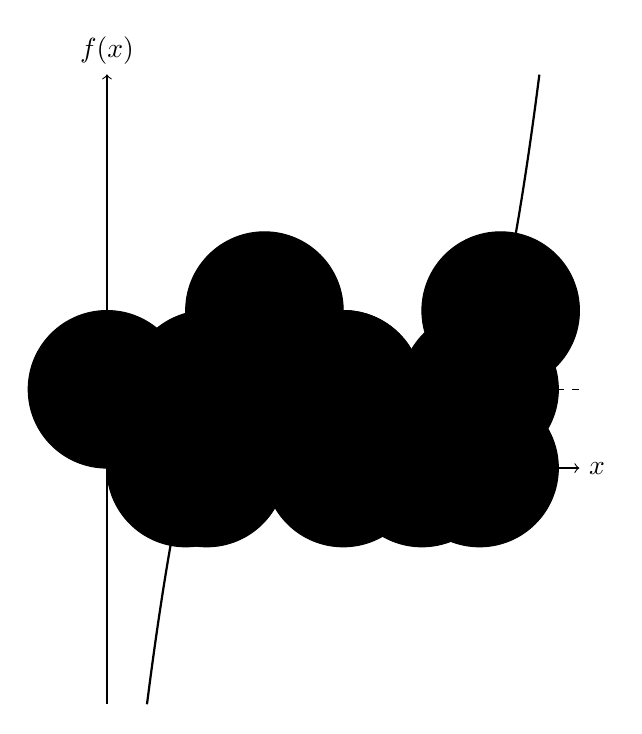
\begin{tikzpicture}
      \draw[->] (0, 0) -- (6, 0) node[right] {$x$};
      \draw[->] (0, -3) -- (0, 5) node[above] {$f(x)$};
      \draw[thick, smooth, samples=100] plot[domain=0.508:5.492] (\x, {((\x)^3 - 9*(\x)^2 + 24*(\x) - 16) / 2});
      \foreach \x/\y/\z in {2/4/above, 4/0/below, 1/0/below left, 5/4/right, 0/2/above right,
      3/2/above right} {
         \filldraw (\x, {\y / 2}) circle (\pointSize) node[\z] {$\left(\x;\y\right)$};
      }
      \foreach \x\y in {1.268/2, 3/2, 4.732/2} {
         \filldraw (\x, {\y / 2}) circle (\pointSize);
         \draw[dashed] (\x, {\y / 2}) -- (\x, 0);
         \filldraw (\x, 0) circle (\pointSize);
      }
      \draw[dashed] (0, 1) -- (6, 1);
   \end{tikzpicture}
   \captionsetup{justification=centering}
   \caption{Dóng điểm để tìm nghiệm với ví dụ $y = 2$}
   \label{fig:ham_so_mot_bien:da_thuc:ddtn}
\end{wrapfigure}

4. Theo đồ thị \ref{fig:ham_so_mot_bien:da_thuc:ddtn} hoặc đồ thị trước đó \ref{fig:ham_so_mot_bien:da_thuc:x3_t9x2_24x_t16}, chúng ta thấy $f$ nhận toàn bộ giá trị trên tập số thực. 

Nếu bạn đọc chỉ vừa mới bước chân vào toán cao cấp, thì để giải bài này bằng đại số có lẽ là một điều khó khăn. Với mọi $y$ thuộc $\mathbb{R}$ thì có \begin{equation}x = \sqrt[3]{\frac{y + \sqrt{y(y-4)}-2}{2}} + \sqrt[3]{\frac{2}{y + \sqrt{y(y-4)}-2}} + 3 \label{eq:ham_so_mot_bien:da_thuc:ddtn}\end{equation}
thỏa mãn $f(x) = y$.

Bạn đọc có thể đã để ý rằng trong công thức tính nghiệm, có căn bậc hai của $\sqrt{y(y-4)}$. Trên tập số thực, $y(y-4) \geq 0$ khi và chỉ khi $y\in\left(-\infty; 0\right]\cup\left[4; \infty\right)$. Viết bằng ngôn ngữ đời thường, $y$ không lớn hơn $0$ hoặc $y$ không nhỏ hơn $4$. Tuy nhiên, mở rộng sang trường số phức thì $\sqrt{y(y-4)}$ vẫn có giá trị, kể cả bên trong dấu khai căn mang dấu âm. Điều hay ở đây là phương trình \ref{eq:ham_so_mot_bien:da_thuc:ddtn} vẫn luôn trả về số thực, tùy theo cách chọn khai căn bậc hai và bậc ba. Để hiểu rõ hơn thì mời bạn đọc tìm hiểu thêm về số phức, giải tích số phức và những vấn đề liên quan.

Về mặt vật lí, thông thường chúng ta sẽ dùng đồ thị để kiểm chứng và cắt giảm phần tính toán đại số. Ví dụ như bài này, chúng ta có thể khẳng định là $f$ nhận toàn bộ giá trị trên tập số thực do nếu lấy một điểm $\left(0; y\right)$ bất kì trên trục tung, dóng ngang tới đồ thị, cắt tại điểm nào thì hoành độ của điểm cắt chính là $x$ để $f(x) = y$. Ở hình \ref{fig:ham_so_mot_bien:da_thuc:ddtn} là ví dụ cho $f(x) = y = 2$.

Trong tương lai, đến khi bạn đọc học về giải tích thì bạn đọc sẽ có cho mình một lập luận xác đáng cho bài tập này.
